\chapter{Resultados e conclusões parciais}
\label{chapterResultados}
%mostrar simulação do painel solar\\
%mostrar mppt\\
%mostrar simulação do buck \\
%mostrar simulação do ci LT8491 com e sem gan
%mostrar optmos da infineon se der pra simular o limite de frequência dos transistores e comparar rdson  e frequência 

\section{Conversor Buck}
%grafico de eficiencia por volts de entrada
%Grafico do indutor por frequencia baseado na tabela. 
\par Os transistores do tipo $GaN$ melhoram a eficiência do circuito quando comparados à mesma topologia utilizando transistores de Si. No gráfico da figura \ref{GrafEficienciaFrequencia} é possivel notar que a topologia com transistores $GaN$ é mais eficiente($\approx 3,5\%$ maior) e isso se deve ao $Rds_{on}$ menor, como mostrado na seção \ref{sectionCap2transistores} e na tabela \ref{t_ComparaTransistor}. O mesmo acontece nas altas frequências: o transitor GaN mantém sua performance com poucas perdas, diferentemente dos transistores de Si.  
\par A escolha da topologia tem bastante influência na eficiência global do conversor. Nota-se um grande ganho de eficência em topologias com dois transistores ao inves de um transistor e um diodo. O diodo $D$ dissipa $P=I_d.V_d$, nos momentos em que conduz ($1-\delta$).
\begin{center}
\begin{figure}[H]
\caption{Eficiência em função da frequência.}
\begin{tikzpicture}
\pgfplotsset{
every axis legend/.append style={ at={(1.05,0.95)}, anchor=north west,legend columns = 1}}
\begin{axis}[
  xlabel=Frequencia em $kHz$,
  ylabel=Eficiência em $\%$]
\addplot table [y=G, x=f]{Freq.dat};
\addlegendentry{GaN+diodo}
\addplot table [y=M, x=f]{Freq.dat};
\addlegendentry{Mosfet+diodo}
\addplot table [y=GG, x=f]{Freq.dat};
\addlegendentry{2xGaN}
\addplot table [y=MM, x=f]{Freq.dat};
\addlegendentry{2xMosfet}
\end{axis}
\end{tikzpicture}
\label{GrafEficienciaFrequencia}
\end{figure}
\end{center}
\par Transistores GaN também possibilitam o aumento a frequencia de chaveamento. O benefício direto do aumento da frequencia de trabalho é a diminuição dos elementos magnéticos e portanto, menor custo. Para a fonte estudada neste trabalho, o indutor mínimo ($L_{min}$) está representado na figura \ref{GrafIndutorFrequencia}. Comparando a frequência mais baixa ($25kHz$ ) e a frequência mais alta ($500kHz$), pode-se diminuir de $100\mu  H$ (18,54mm x 15,24mm x 7,11mm) para $5,6\mu H$ (4,7mm x 4,2mm x 3,45mm), além da redução de $\approx 60\%$ no custo médio/componente.
\begin{center}
\begin{figure}[H]
\caption{Eficiência em função da frequência.}
\begin{tikzpicture}
\pgfplotsset{
every axis legend/.append style={ at={(1.05,0.95)}, anchor=north west,legend columns = 1}}
\begin{axis}[
  xlabel=Frequencia em $kHz$,
  ylabel=Indutância em $\mu H$]
\addplot table [y=L, x=f]{L.dat};
\addlegendentry{$V_{in}=17V$; $\delta=25\%$}
\end{axis}
\end{tikzpicture}
\label{GrafIndutorFrequencia}
\end{figure}
\end{center}
\par As simulações também comtemplam a variação da tensão de saída do painel solar fotovoltaico, uma vez que tensão de saída e corrente maxima podem variar de acordo com nível de iluminação disponível. A eficiência em relação à tensão $V_{in}$ está no gráfico da figura \ref{GrafEficienciaTensao}. 
\begin{center}
\begin{figure}[H]
\caption{Eficiência em função da tensão}
\begin{tikzpicture}
\pgfplotsset{
every axis legend/.append style={ at={(1.05,0.95)}, anchor=north west,legend columns = 1}}
\begin{axis}[
  xlabel=Tensão em $V$,
  ylabel=Eficiência em $\%$]
\addplot table [y=GD, x=T]{tensao.dat};
\addlegendentry{GaN+Diodo}
\addplot table [y=MD, x=T]{tensao.dat};
\addlegendentry{Mosfet+Diodo}
\addplot table [y=2G, x=T]{tensao.dat};
\addlegendentry{2xGaN}
\addplot table [y=2M, x=T]{tensao.dat};
\addlegendentry{2xMosfet}
\end{axis}
\end{tikzpicture}
\label{GrafEficienciaTensao}
\end{figure}
\end{center}
\par A tensão de saída das fontes está na figura \ref{fig:BuckVoAll}. Nota-se menor $\Delta V$ nas topologias com frequência maior, e a tensão de saída $V_o$ mais proxima da nominal ($4.3V$) nas topologias com dois diodos, uma vez que o diodo proporciona uma queda de $\approx 0,7V$ (o duty-cycle $\delta$ não foi recalculado para manter a comparação de eficiência). 
\par Os testes até o momento são em \textit{open loop}, com foco em dois parametros: $Rds_{on}$ e frequência.

\begin{figure}[H]
\centering
\caption{Tensão de saída $V_o$, \textit{open loop}, com variação da Frequência e Indutor.}
\subfloat[][GaN+Diodo]{
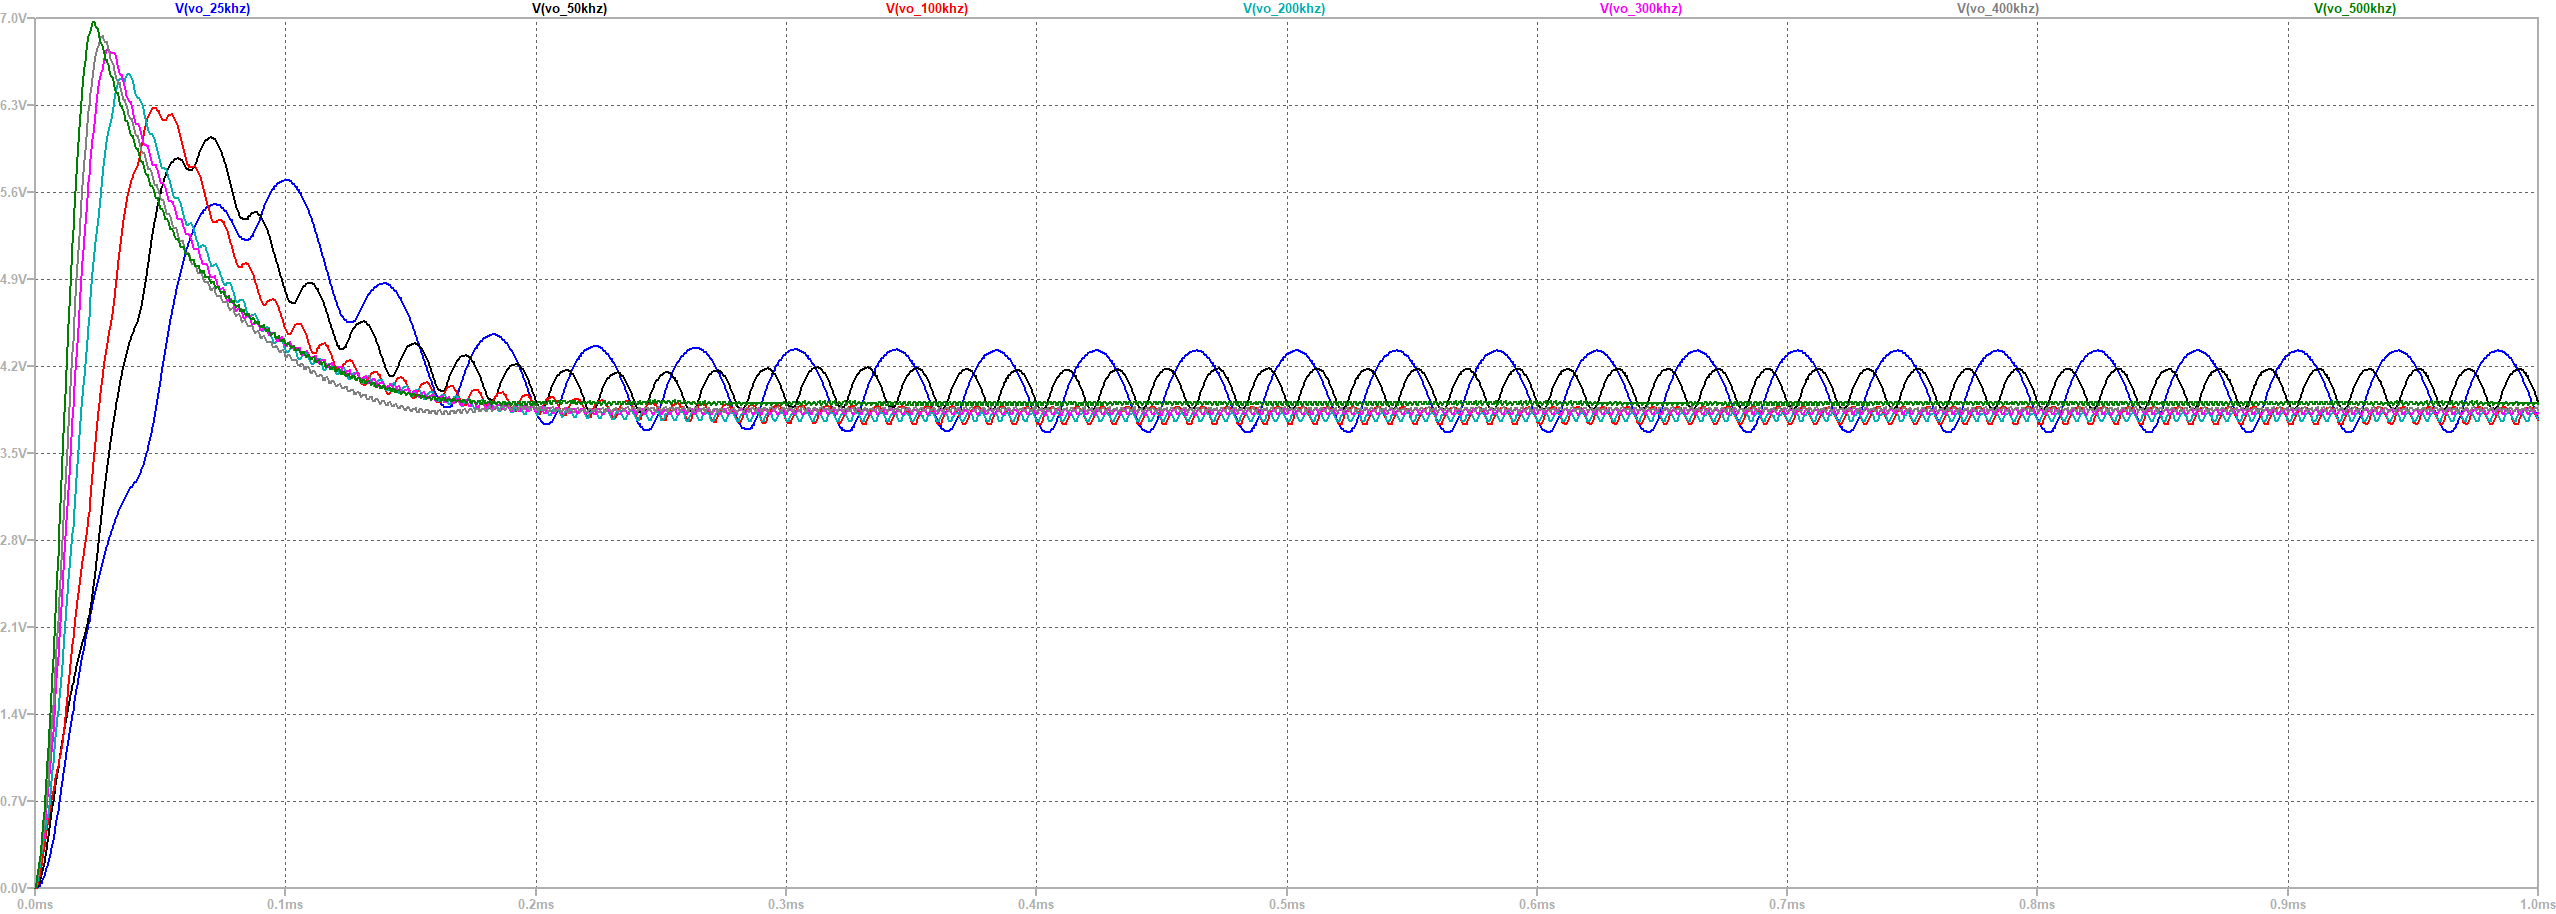
\includegraphics[width=0.5\textwidth]{figuras/Vo_Buck_Gan_Diodo.png} 
\label{fig:subfig1}}
\subfloat[][2xGaN]{
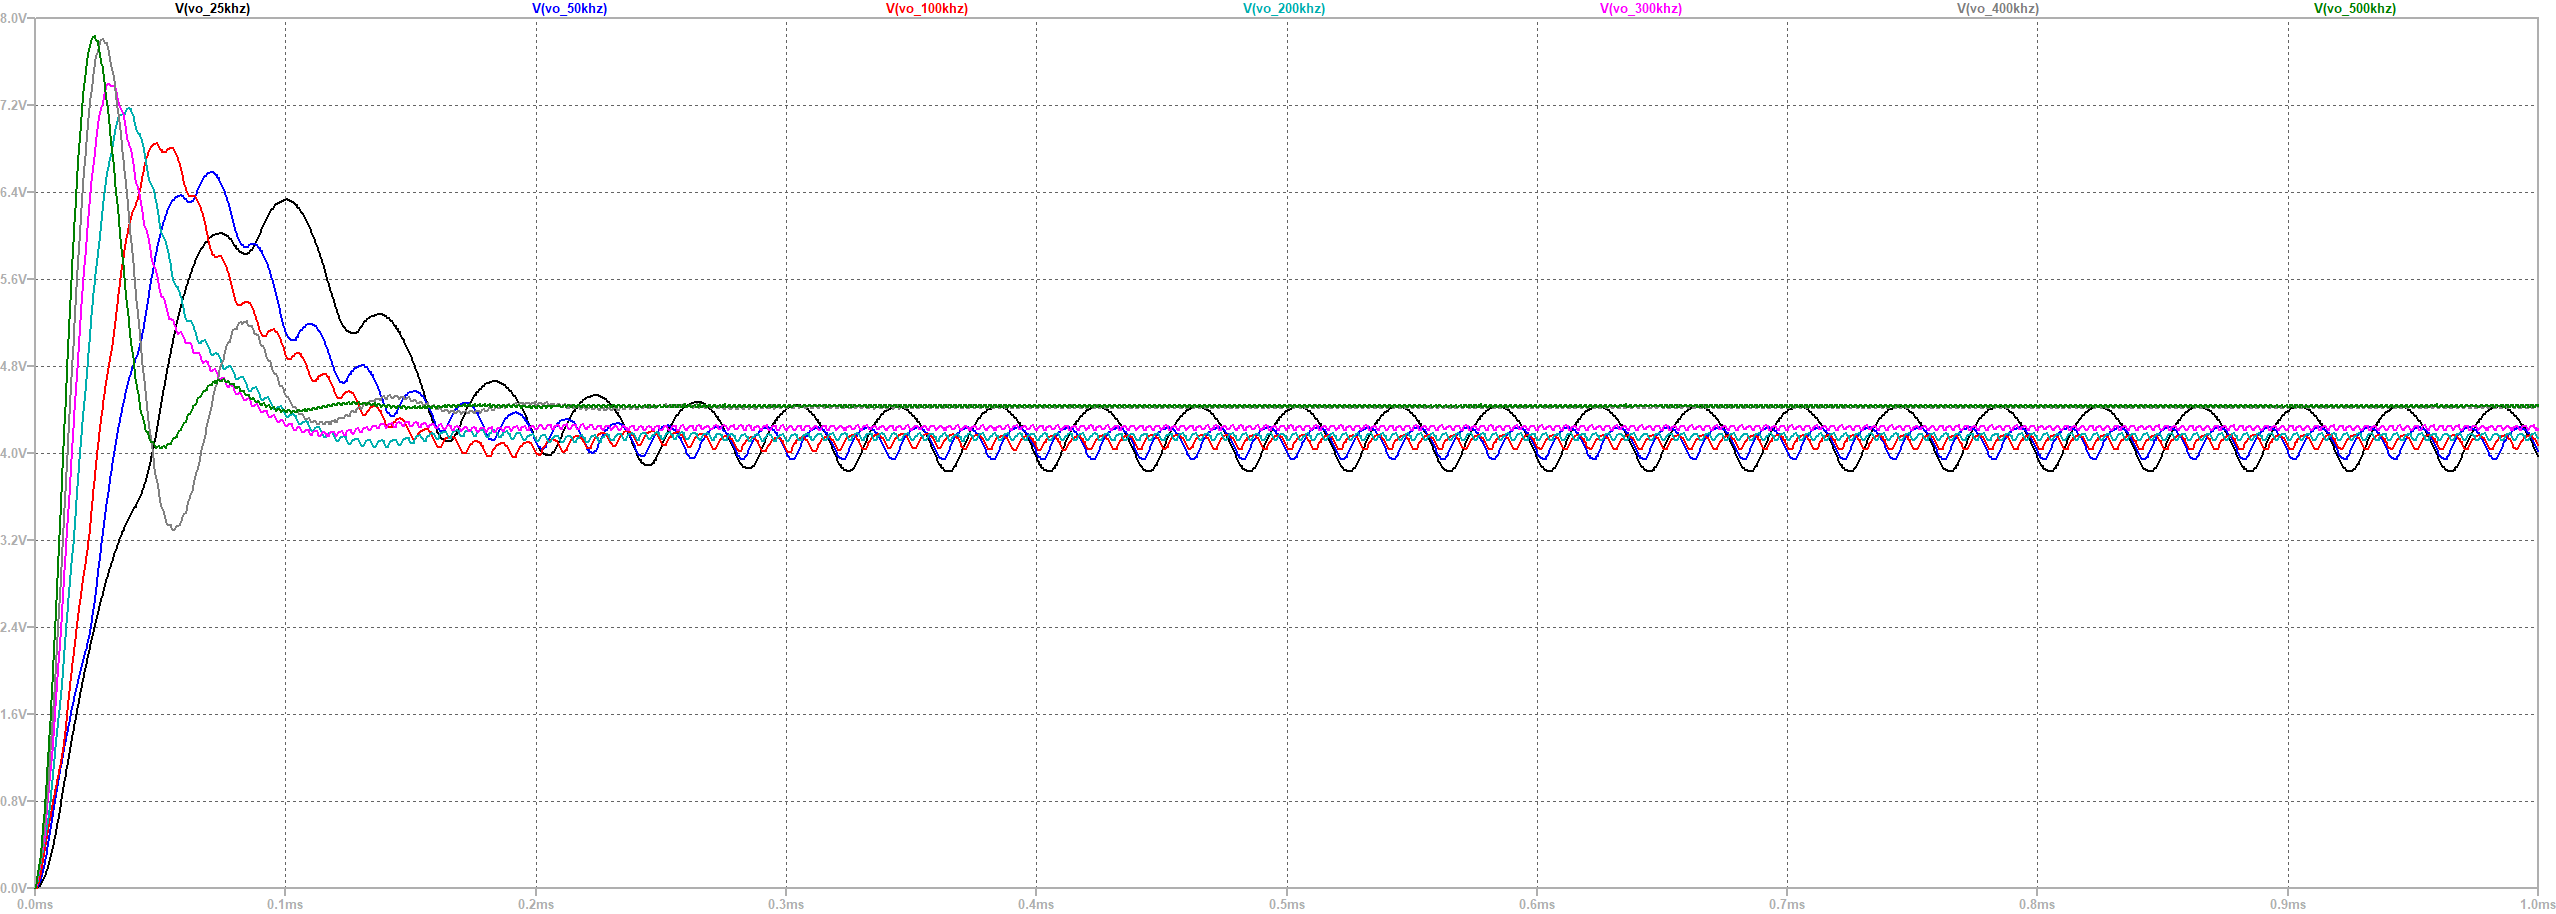
\includegraphics[width=0.5\textwidth]{figuras/Vo_Buck_Gan_Gan.png} 
\label{fig:subfig2}}
\qquad
\subfloat[][Mosfet+Diodo]{
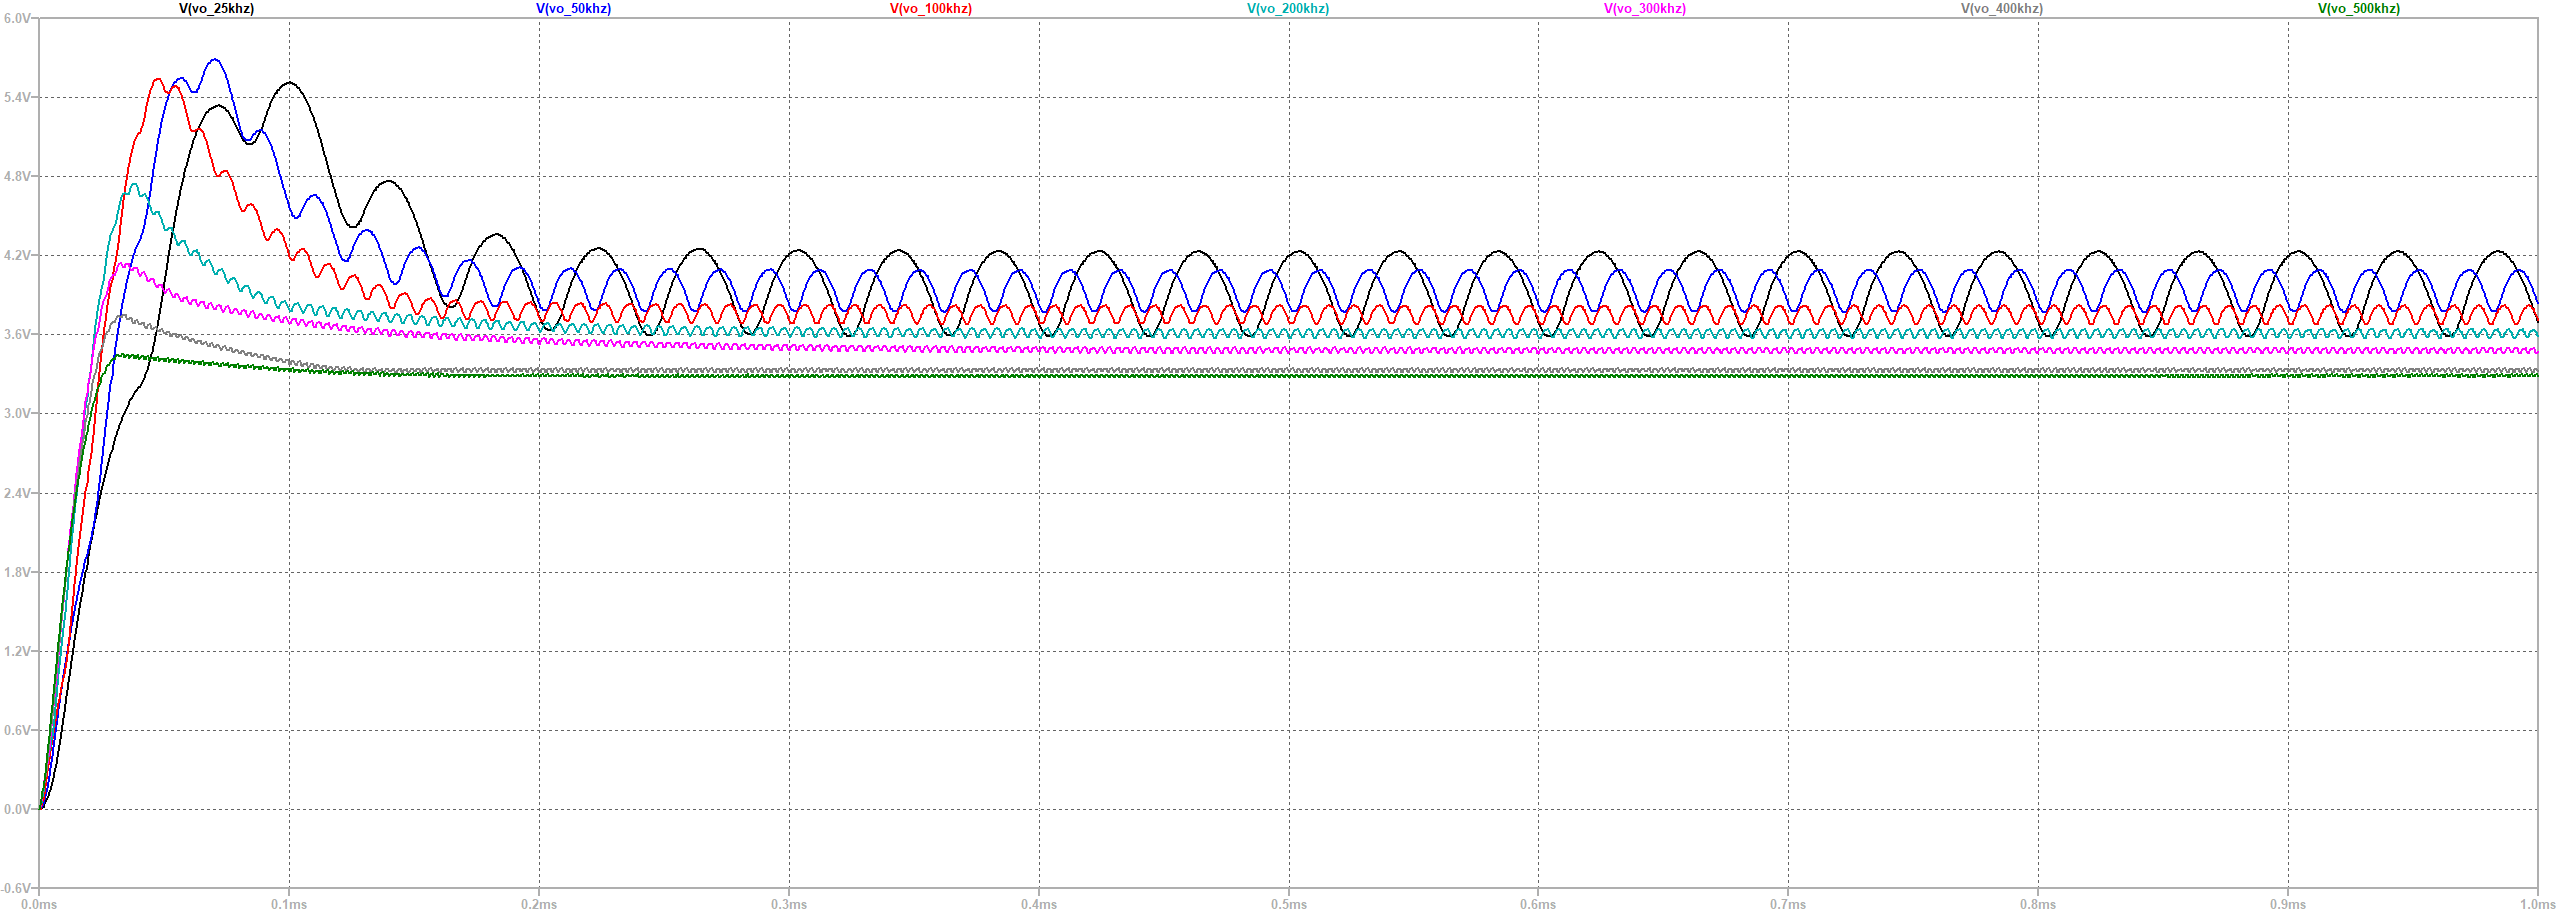
\includegraphics[width=0.5\textwidth]{figuras/Vo_Buck_Mosfet_Diodo.png} 
\label{fig:subfig3}}
\subfloat[][2xMosfet]{
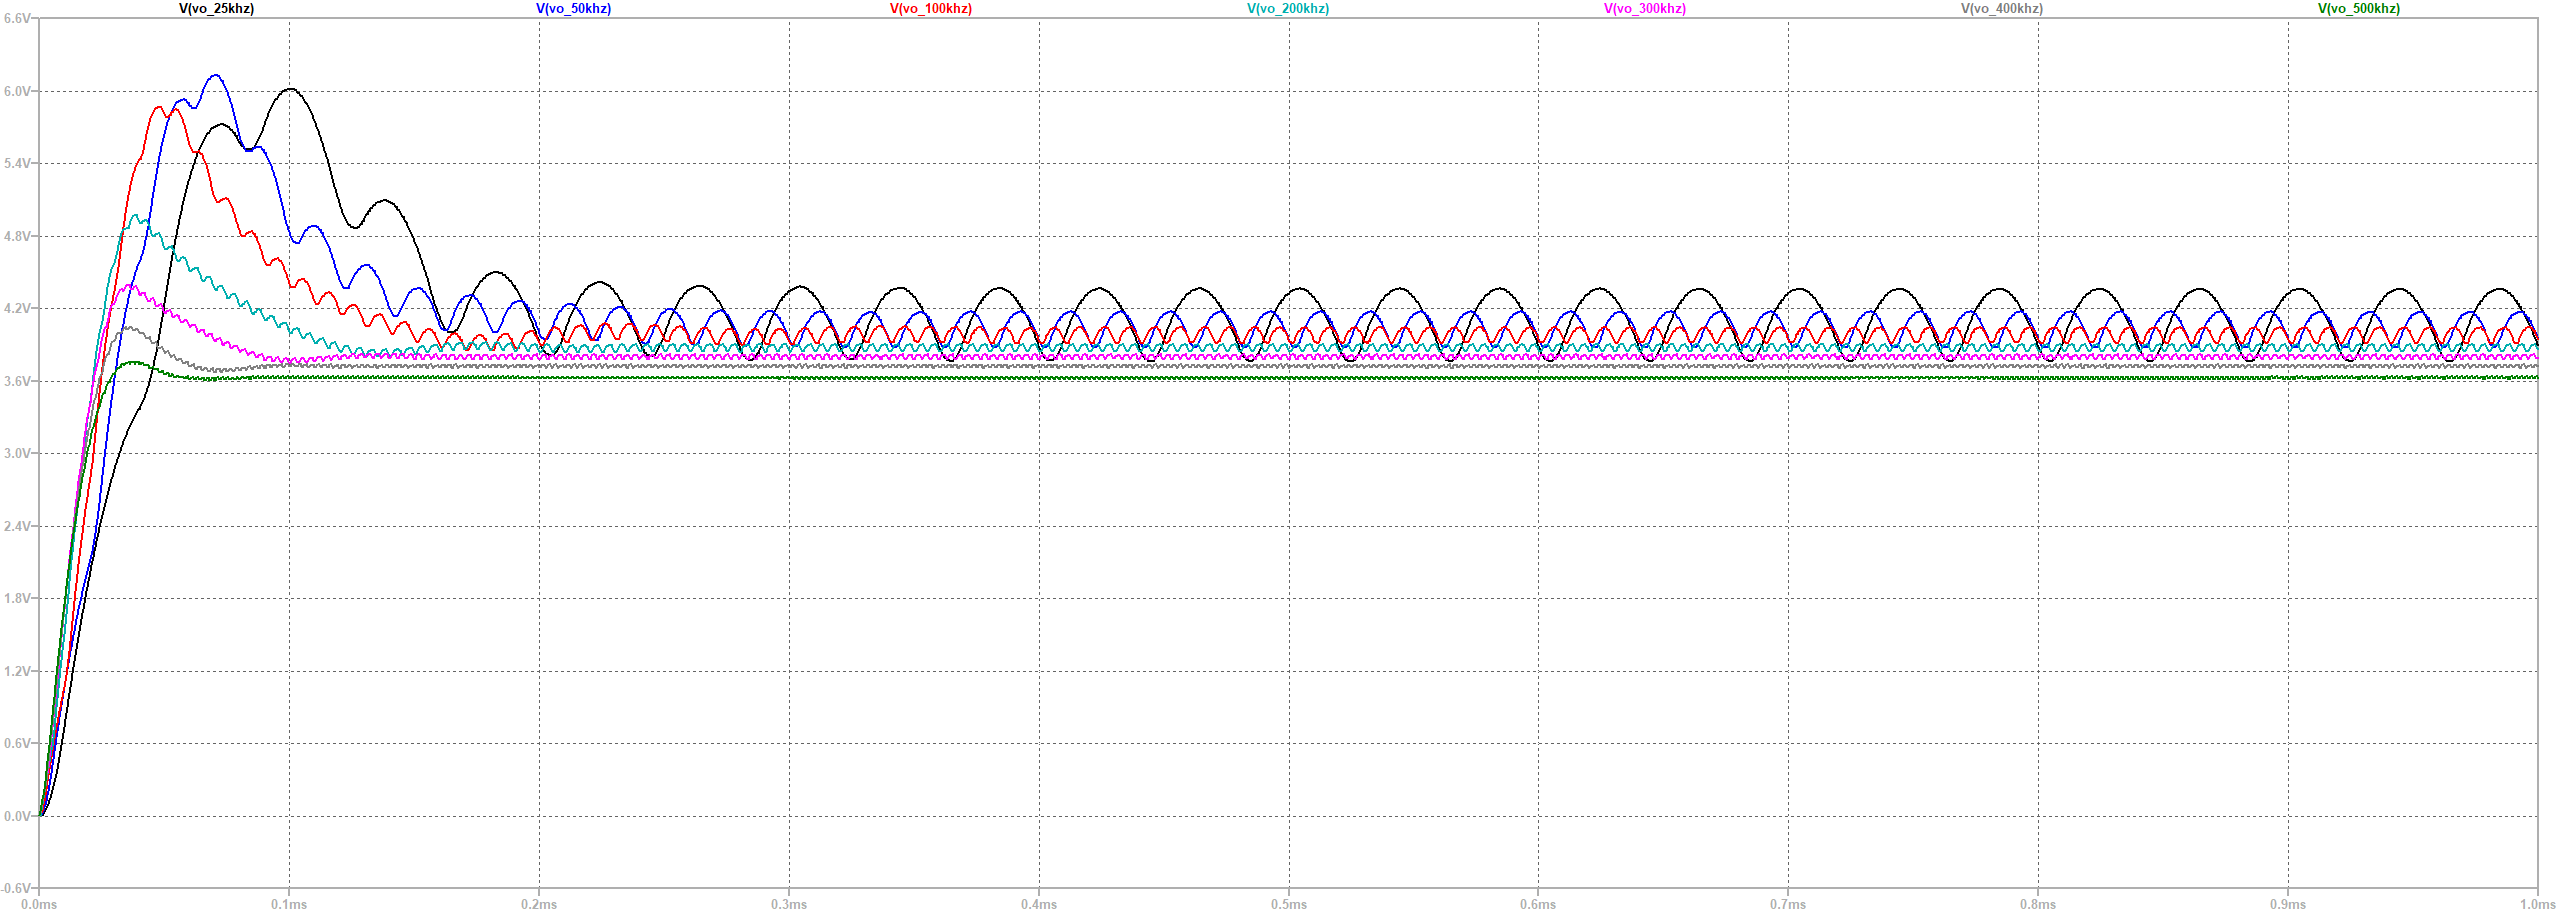
\includegraphics[width=0.5\textwidth]{figuras/Vo_Buck_Mosfet_Mosfet.png} 
\label{fig:subfig4}}
\label{fig:BuckVoAll}
\end{figure}

\section{Painel solar fotovoltaico}
A simulação do Painel solar está representada na figura \ref{FigPV} e pode ser comparada com a tabela \ref{t_PV}. Os parâmetros de Potência máxima($P_{max}=V_m.I_m$) estão bem representados nesta simulação. $V_m \approx 17V$ e $I_{m} \approx 0.6A$ coincidem com $P_{max}$ simulado e o apresentado pelo fabricante.
\par A tensão de circuito aberto ($V_{oc}$) não está representada adequadamente e deve sofrer reajustes no modelo.
\begin{figure}[H]
\caption{Simulação painel solar fotovoltáico}
 \centering % para centralizarmos a figura
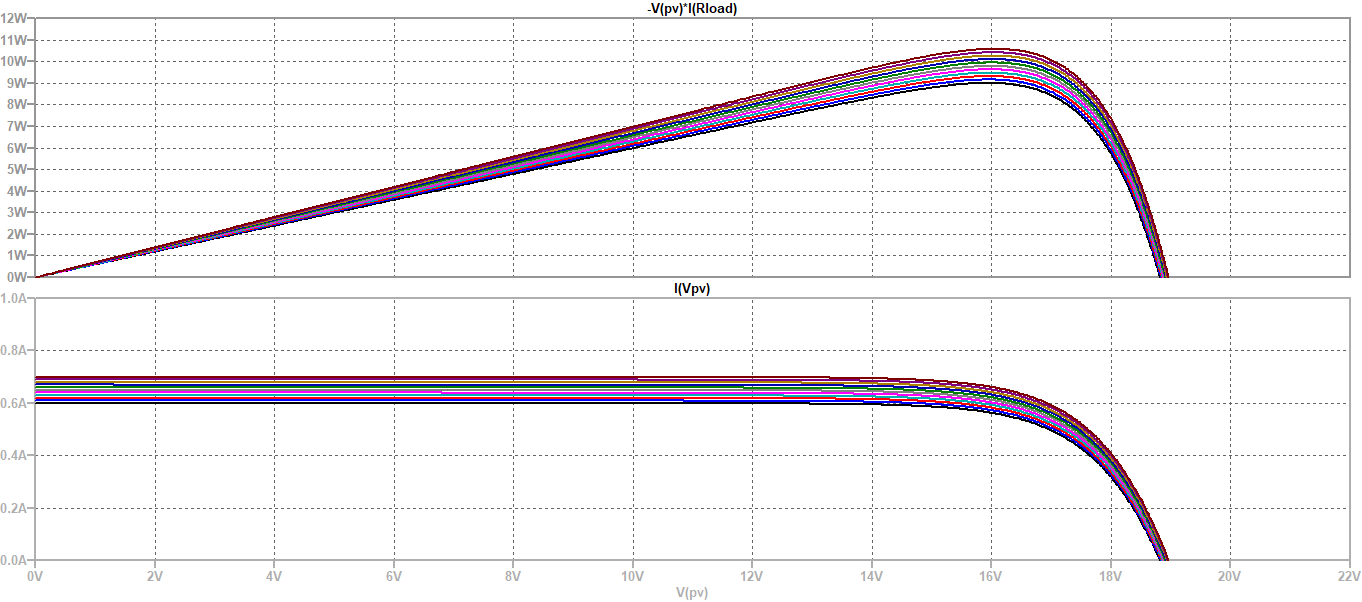
\includegraphics[width=14cm]{figuras/PV_resultados.png} 
\label{FigPV}
\end{figure}
